\documentclass[10pt]{beamer}

\usetheme[progressbar=frametitle]{metropolis}
\usepackage{appendixnumberbeamer}
\usepackage{graphicx}
\usepackage{booktabs}
\usepackage[scale=2]{ccicons}
\usepackage[font=footnotesize,labelfont=bf]{caption}
\usepackage{mwe}

\usepackage{pgfplots}
\usepgfplotslibrary{dateplot}

\usepackage{xspace}
\newcommand{\themename}{\textbf{\textsc{metropolis}}\xspace}

\title{Arabic Mathematics}
\subtitle{Al-Kashi's Method for sin($1^{\circ}$)}
% \date{\today}
\date{}
\author{Stefano Fochesatto}

\begin{document}

\maketitle

\begin{frame}{Jamshid al-Kashani}
  \begin{columns}[T]
    \begin{column}{.60\textwidth}
   
      \begin{itemize}
        \item Born around 1380 in Kashan, Iran.
        \item Was a prominent member, and later the leader of the Samarkand Observatory.
        \item A prodigious calculator, his work largely involved producing more precise trigonometric tables. 
        \item First methodical approach to our modern decimal notation. (vertical line)
        \item Law of Cosines
      \end{itemize}

    \end{column}
    \begin{column}{.40\textwidth}
  % Your image included here
  \begin{figure}
    \begin{center}
      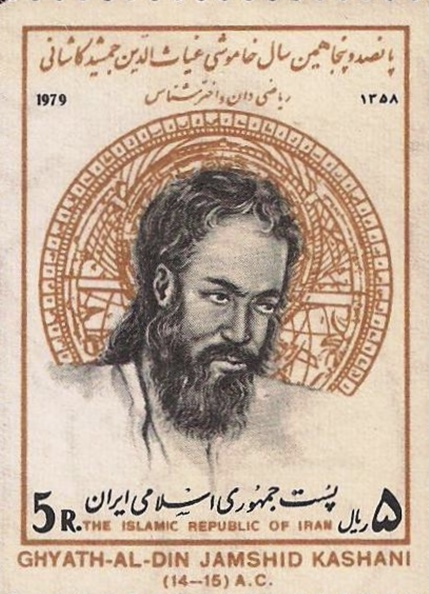
\includegraphics[width=.75\textwidth]{samarkand.jpg}
    \caption{Depiction of Al-Kashi from MathStamps}
    \end{center}
  \end{figure}
      \end{column}

 
    
  \end{columns}
\end{frame}

\begin{frame}{Motivation for sin($1^{\circ}$)}
  \begin{itemize}
    \item Recall that trigonometric tables were made incrementally. 
    \item Ptolemy's Construction
    \begin{itemize}
      \item Pythagorean special right triangles: 30,45,60
      \item Elements Book 4 Proposition 10: 36,72,54,18
      \item Half Angle 54: 27
      \item Angle Difference 30-27: 3
      \item Half Angle 3 : 1.5 , 0.75
      \item Finally sin(1) is approximated 
    \end{itemize}
    \item Precise incremental unit $\to$ precise table
    \item Astronomy requires precise trig tables. 
  \end{itemize}
\end{frame}

\begin{frame}{Al-Kashi's Method: The Setup}
  \begin{itemize}
    \item First he discovered the triple angle identity (Mixture of construction and trig identity).
    \begin{equation*}
      sin(3\theta) = 3sin(\theta) - 4sin^3(\theta) 
    \end{equation*}
    \item Substitute $\theta = 1$ and $sin(1) = x$ and we get a cubic,
    \begin{equation*}
      sin(3) = 3x - 4x^3.
    \end{equation*}
    \item Solve for $x$,
    \begin{equation*}
      x = \frac{4}{3}x^3 + \frac{1}{3} sin(3).
    \end{equation*}
    \item Now we have a function to iterate over.
    \item Arbitrary precision.
  \end{itemize}

\end{frame}

\begin{frame}{Al-Kashi's Method: Iteration Step}
  \begin{itemize}
    \item Al-Kashi knew that $sin(1) \approx \frac{1}{3} sin(3)\approx .01$
    \begin{itemize}
      \item Let $x_0 = .01$
    \end{itemize}
    \item Suppose that $x = .01d_1d_2d_3d_4d_5\dots$ where $0 \leq d_i \leq 9$.
    \item Substituting into our function we get,
    \begin{equation*}
      .01d_1d_2d_3d_4d_5\dots = \frac{4}{3}(.01d_1d_2d_3d_4d_5\dots)^3 + \frac{1}{3} sin(3).
    \end{equation*}
    \item Subtract $x_0$ from both sides,
    \begin{equation*}
      .00d_1d_2d_3d_4d_5\dots = \frac{4}{3}(.01d_1d_2d_3d_4d_5\dots)^3 + (\frac{1}{3} sin(3) - .01).
    \end{equation*}
    \item Note that,
      \begin{equation*}
        \frac{1}{3} sin(3) - .01 = .007445
      \end{equation*}
      \begin{equation*}
        \frac{4}{3}(.01d_1d_2d_3d_4d_5\dots)^3 = \frac{4}{3}(.000001d_1d_2d_3d_4d_5\dots)
      \end{equation*}
      \item Thus $d_1 = 7$, set $x_1 = .017$ and repeat.
  \end{itemize}
\end{frame}

\begin{frame}{Al-Kashi's Method: Results}
  \begin{itemize}
    \item With this method Al-Kashi calculated,
    \begin{equation*}
      sin(1) =  0.017452406437283510
    \end{equation*}
    \item 18 digits vs 16 digits with IEEE Double Precision 
    \item Phone calculator demo
  \end{itemize}
\end{frame}

\begin{frame}{Comparison to Modern Methods: Power Series}
  \begin{itemize}
    \item Recall the power series of $sin$,
    \begin{equation*}
      sin(x) = x - \frac{x^3}{3!} + \frac{x^5}{5!} - \frac{x^7}{7!} + \dots
    \end{equation*}
    \item Matlab Demo
  \end{itemize}
\end{frame}




\begin{frame}{Comparison to Modern Methods: Counting FLOPs}
  \begin{itemize}
    \item Al-Kashi
    \begin{itemize}
      \item $\sim 7n$ operations  = $O(n)$ 
    \end{itemize}
    \item Power Series 
    \begin{itemize}
      \item $\sim 4n^2 - 2n - 1$ operations = $O(n^2)$
    \end{itemize}
  \end{itemize}
\end{frame}




\end{document}
